%%%%%%%%%%%%%%%%%%%%%%%%%%%%%%%%%%%%%%%%%
% University Assignment Title Page 
% LaTeX Template
% Version 1.0 (27/12/12)
%
% This template has been downloaded from:
% http://www.LaTeXTemplates.com
%
% Original author:
% WikiBooks (http://en.wikibooks.org/wiki/LaTeX/Title_Creation)
%
% License:
% CC BY-NC-SA 3.0 (http://creativecommons.org/licenses/by-nc-sa/3.0/)
% 
% Instructions for using this template:
% This title page is capable of being compiled as is. This is not useful for 
% including it in another document. To do this, you have two options: 
%
% 1) Copy/paste everything between \begin{document} and \end{document} 
% starting at \begin{titlepage} and paste this into another LaTeX file where you 
% want your title page.
% OR
% 2) Remove everything outside the \begin{titlepage} and \end{titlepage} and 
% move this file to the same directory as the LaTeX file you wish to add it to. 
% Then add \input{./title_page_1.tex} to your LaTeX file where you want your
% title page.
%
%%%%%%%%%%%%%%%%%%%%%%%%%%%%%%%%%%%%%%%%%
%\title{Title page with logo}
%----------------------------------------------------------------------------------------
%	PACKAGES AND OTHER DOCUMENT CONFIGURATIONS
%----------------------------------------------------------------------------------------

\documentclass[12pt]{article}
\usepackage[english]{babel}
\usepackage[utf8x]{inputenc}
\usepackage{amsmath}
\usepackage{graphicx}
\usepackage{caption}
\usepackage{amssymb}
\usepackage{enumitem}
\usepackage[colorinlistoftodos]{todonotes}

\begin{document}

\begin{titlepage}

\newcommand{\HRule}{\rule{\linewidth}{0.5mm}} % Defines a new command for the horizontal lines, change thickness here

\center % Center everything on the page
 
%----------------------------------------------------------------------------------------
%	HEADING SECTIONS
%----------------------------------------------------------------------------------------

\textsc{\LARGE University of California, Los Angeles}\\[1.5cm] % Name of your university/college
\textsc{\Large M152A Lab2}\\[0.5cm] % Major heading such as course name
 

%----------------------------------------------------------------------------------------
%	TITLE SECTION
%----------------------------------------------------------------------------------------

\HRule \\[0.4cm]
{ \huge \bfseries Floating Point Conversion}\\[0.4cm] % Title of your document
\HRule \\[1.5cm]
 
%----------------------------------------------------------------------------------------
%	AUTHOR SECTION
%----------------------------------------------------------------------------------------

\begin{minipage}{0.4\textwidth}
\begin{flushleft} \large
\emph{Group Members:}\\
Chengyu Wang\\
Simeng Pang\\
Yaowei Guo% Your name
\end{flushleft}
\end{minipage}
~
\begin{minipage}{0.4\textwidth}
\begin{flushright} \large
\emph{TA:} \\
Jia Guo % Supervisor's Name
\end{flushright}
\end{minipage}\\[4cm]

% If you don't want a supervisor, uncomment the two lines below and remove the section above
%\Large \emph{Author:}\\
%John \textsc{Smith}\\[3cm] % Your name

%----------------------------------------------------------------------------------------
%	DATE SECTION
%----------------------------------------------------------------------------------------

{\large \today}\\[2cm] % Date, change the \today to a set date if you want to be precise

%----------------------------------------------------------------------------------------
%	LOGO SECTION
%----------------------------------------------------------------------------------------

%\includegraphics{logo.png}\\[1cm] % Include a department/university logo - this will require the graphicx package
 
%----------------------------------------------------------------------------------------

\vfill % Fill the rest of the page with whitespace

\end{titlepage}

\newpage
\section*{Introduction}
This lab is about converting a 12-bit twos-complement integer to an 8-bit floating point number. The converted floating point number consists of three parts: a sign bit, three exponent bits and four significand bits.\\
\begin{minipage}{\linewidth}
            \centering
            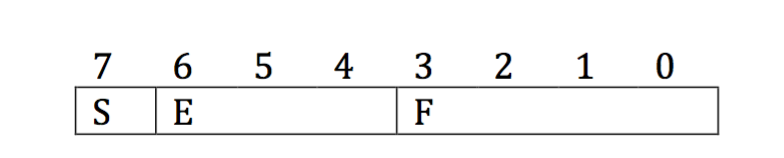
\includegraphics[width=10cm, height=1.5cm]{float-representation.png}
           % \captionof{figure}{Output Waveforms}
           % \label{fig:figure1}
        \end{minipage}
The value represented by this 8-bit number is:
$$ V = (-1)^S * F * 2^E$$

\section*{Design}
There is only one module called FPCVT in this project. In this module, there are 4 steps: 
\begin{itemize}
	\item Determine the sign bit
	\item Determine the exponent field
	\item Determine the significand filed with rounding 
	\item Most negative number case
\end{itemize}

\begin{minipage}{\linewidth}
            \centering
            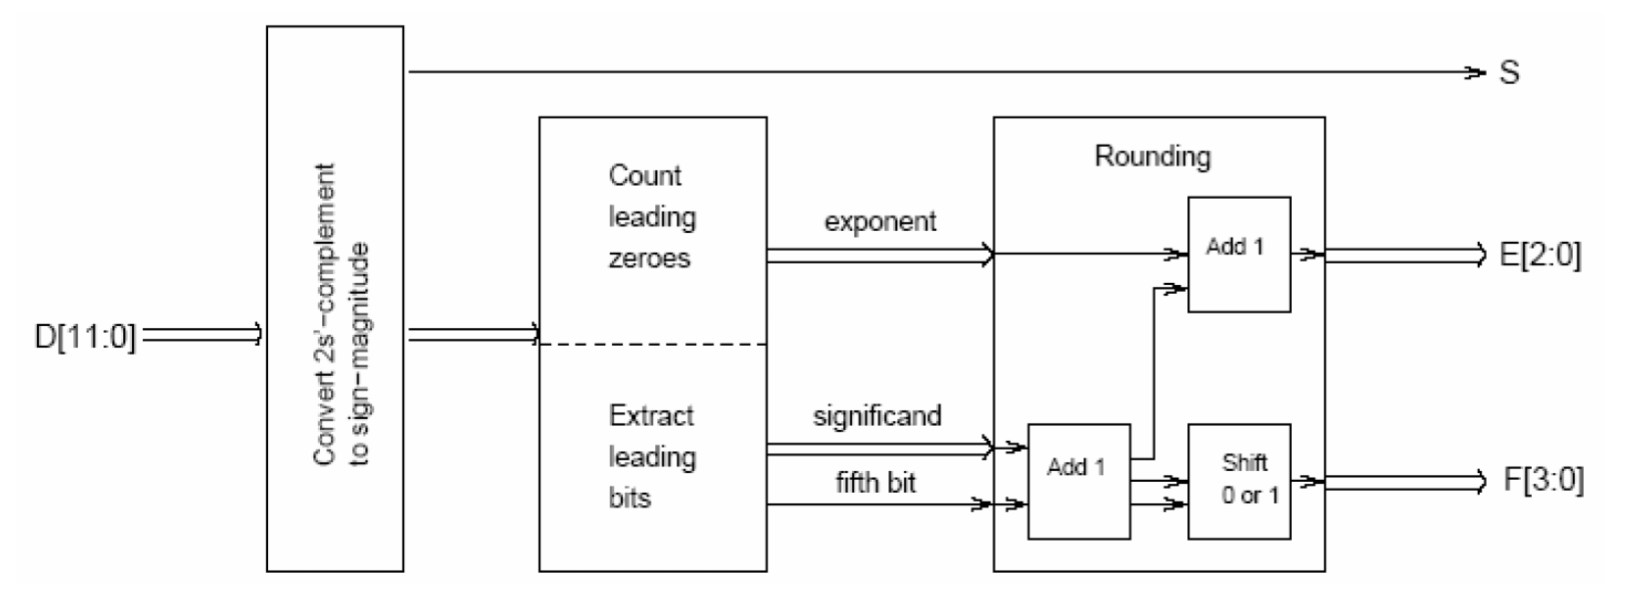
\includegraphics[width=15cm, height=5.5cm]{design.png}
            \captionof{figure}{Overall design diagram from lab manual}
            \label{fig:figure2}
        \end{minipage}

\subsection*{Sign bit}
Sign bit is the most significant bit of the 12-bit input number.
The code goes as follows:
$$S = D[11]$$

\subsection*{Exponent bit}
To count the leading zeroes of the input, the first step is to convert the twos-complement number to the number of its absolute value. The code goes as follows:
$$tmp = \sim D + 1$$
We have a table of the relationship between leading zeroes of $tmp$ and the exponent filed. \\
\begin{minipage}{\linewidth}
            \centering
            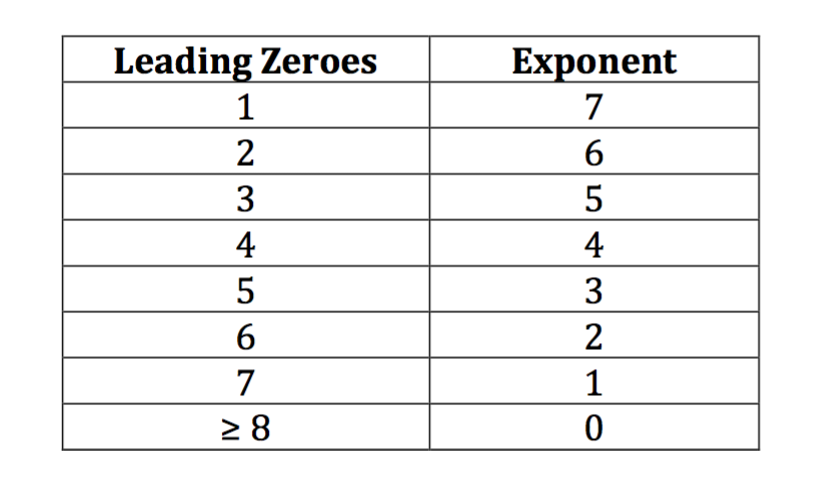
\includegraphics[width=10cm, height=5cm]{lead_zerotable.png}
           % \captionof{figure}{Output Waveforms}
           % \label{fig:figure1}
        \end{minipage}
According to this table, we can get the exponent field of 3 bits. 

\subsection*{Significand and Rounding}
There are two cases to consider here: less than 8 leading zeroes or not.\\
When there are  8 or more leading zeroes, the exponent will be 0. So we simply need to take the 4 least significant bits.
$$\hspace{-8cm} F = newtmp [11:8]$$
When there are less than 8 leading zeroes, we first take the four bits following the last leading zero as the significand. The code goes as follows:
$$\hspace{-6cm} newtmp = tmp << lead\_zero;$$
$$\hspace{-8cm} F = newtmp [11:8];$$
Then we use the fifth bit following the last leading zero to judge whether there is rounding. If the fifth bit $(newtmp[7])$ is 0, the nearest number can be obtained by truncating-simply using the first four bits. If the fifth bit is 1, the nearest number is obtained by rounding up-adding 1 to the first four bits.\\
When rounding up happens, there are three cases:
\begin{itemize}
	\item The four bits are not 1111. After adding one to the four bits, no overflow happens. Then we use the result after addition as the significand.
	\item The four bits are 1111 and the exponent bits are not 111. After adding one to the four bits, there is overflow.
	$$1111 + 1 = 10000$$
	This problem is solved by right shift the significand by 1 bit and get 1000. Meanwhile, exponent will increase by 1 to compensate. The code goes as follows(Decimal value corresponding to the bit string is used in the code):
	$$\hspace{-8cm}if( F == 15)$$
	$$ \hspace{-9.3cm} begin $$
	$$ \hspace{-8cm}  F = 8;$$
	$$	\hspace{-7.4cm}if(E != 7)$$
	$$	\hspace{-7.4cm} E=E+1;$$
	
	\item The four bits are 1111 and exponent bits are 111. If exponent increases by 1, there will be exponent overflow. So, we change nothing in this case. 
\end{itemize}

\subsection*{Most negative number case }
When the input is 100000000000, the most negative number that can be represented within 12 bits, the leading zeroes counted will be 0. 
$$ \sim 100000000000 + 1 = 100000000000$$
In this case we simply give the exponent and the significand the largest possible values(111 and 1111, in decimal value 7 and 15). 
$$\hspace{-7cm}if(D == 12'b100000000000)$$
$$\hspace{-9.6cm}	begin$$
$$\hspace{-8cm}	 E = 7;$$
$$\hspace{-8cm}	 F = 15;$$
$$\hspace{-9.8cm}	end$$

\section*{Simulation Document}
In this section we cover many possible 12-bit input cases, D, and show the outputs S, E and F. We consider the normal cases and edges cases and check that if they satisfy the rounding requirement.
\\
\\
Test Cases:
\\
D = 12'b100000000000;  
\\
S:1, E:111, F:1111       //this is the smallest number we can test, since negating this number gives the same number, we have to treat this as a special case.
\\
\\
D = 12'b000000101100;
\\
S:0, E:010 F:1011        //this is the normal case
\\
\\
D = 12'b000110110000;
\\
S:0, E:101, F:1110       //this is the case when we have to round up F because there is a 1 following the truncated number, so we change 1101 to 1110 for F.
\\
\\
D = 12'b000001111101;
\\
S:0, E:100, F:1000       //this is the special case for rounding. Since we can only take four bits for F, we have to consider the fifth significant number. Since it's 1, we have to round up. At the same time E should also add one.
\\
\\
D = 12'b011111000000;
\\
S:0, E:111, F:1111       //this is the special case when F needs to round up but E has already reached its biggest number, so we can just keep both E and F with their largest representation.
\\
\\
D = 12'b111111111111;
\\
S:1, E:000, F:0001       //this is the negative number conversion. We first converted it to positive representation using two's complement, then we just set S to 1 and do the normal conversion.
\\
\\
D = 12'b000000000000;
\\
S:0, E:000, F:0000       //this is representation of 0, so S,E and F are all zero.
\\
\\
D = 12'b111111110000;
\\
S:1, E:001, F:1000       //this is also a negative number conversion.
\\
\\
D = 12'b011111001010;     
\\
S:0, E:111 F:1111        //this is also the special case that the number needs to be round up but E and F both reach the biggest number, so we just keep E and F as before.
\\
\\
D = 12'b100000011111;
\\
S:0, E:111, F:1111       //this is the negative number case that after converting it using two's complement, both E and F reach the largest number and we don't need to round up then. \\

\begin{minipage}{\linewidth}
            \centering
            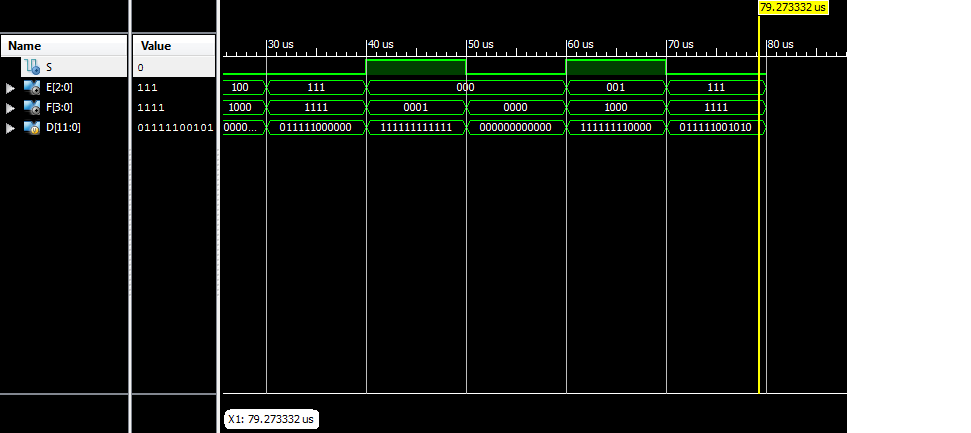
\includegraphics[width=13cm, height=7.5cm]{lab2.png}
            \captionof{figure}{Output simulation waveforms of some testcases}
            \label{fig:figure2}
        \end{minipage}




\end{document}